\section{Design and Implementation}
After the interview with Tove there was some changes to be implemented.
The new requirements are mentioned in \cref{sprint4:requirement_table} and the changes made to satisfy these requirements will be described in this section.
Additionally, due to a change in the way the active profile is changed, a new profile-selector button was added to the main menu.

\begin{figure}
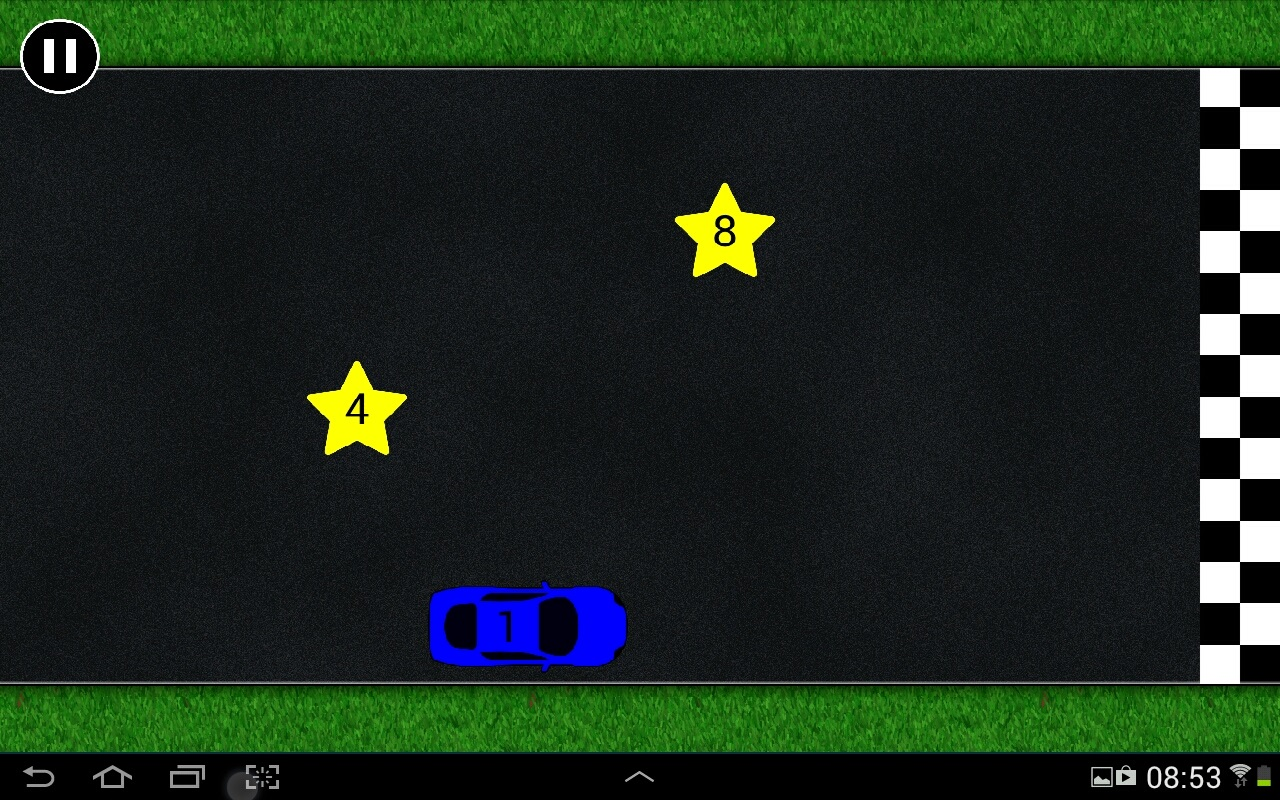
\includegraphics[width=\textwidth]{game}
\caption{The game with a finishing line as goal}
\label{game_with_finishing_line}
\end{figure}

\subsection{Game objective}\label{s4_gameobjective}
According to \cref{sprint4_objective} (see \cref{sprint4:requirement_table}) the garages had to be removed from the game and replaced with a simple finishing line.
The game also had to be changed so the items on the road had to be collected instead of avoided.
These changes introduced some changes to the logic on how to determine when the player wins.
Now it is necessary for the player to collect all items before reaching the finishing line. 
The new appearance can be seen on \cref{game_with_finishing_line}, where the new star model for items is also depicted.
This new model was introduced to be able to distinguish the two game modes from each other.
Choosing between the two modes was implemented in settings as seen on \cref{gamemode}


\begin{figure}
\begin{subfigure}{0.5\textwidth}
\centering
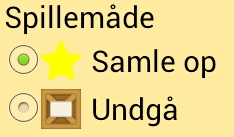
\includegraphics{GameModeChooser}
\caption{Choosing gamemode}
\label{gamemode}
\end{subfigure}
~
\begin{subfigure}{0.5\textwidth}
\centering
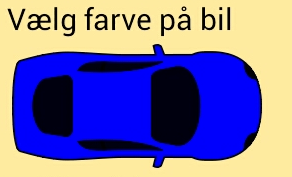
\includegraphics{CarColorPicker}
\caption{Changing the color of the car}
\label{carcolor}
\end{subfigure}
\caption{Changes in settings}
\label{Settings}
\end{figure}

Because of the change away from garages it is now only necessary to choose one color for the game. 
This change was reflected in settings by only showing one colorpicker and shaping this like a car.
This car changes color according to the picked color and can be seen on \cref{carcolor}

The calibration fragment was changed slightly to blend more into the other components of the settings screen. 
A text was added to make the usage of the fragment more clear for the users.
The changed fragment as well as the complete settings screen can be seen on \cref{settings_s4}

\begin{figure}
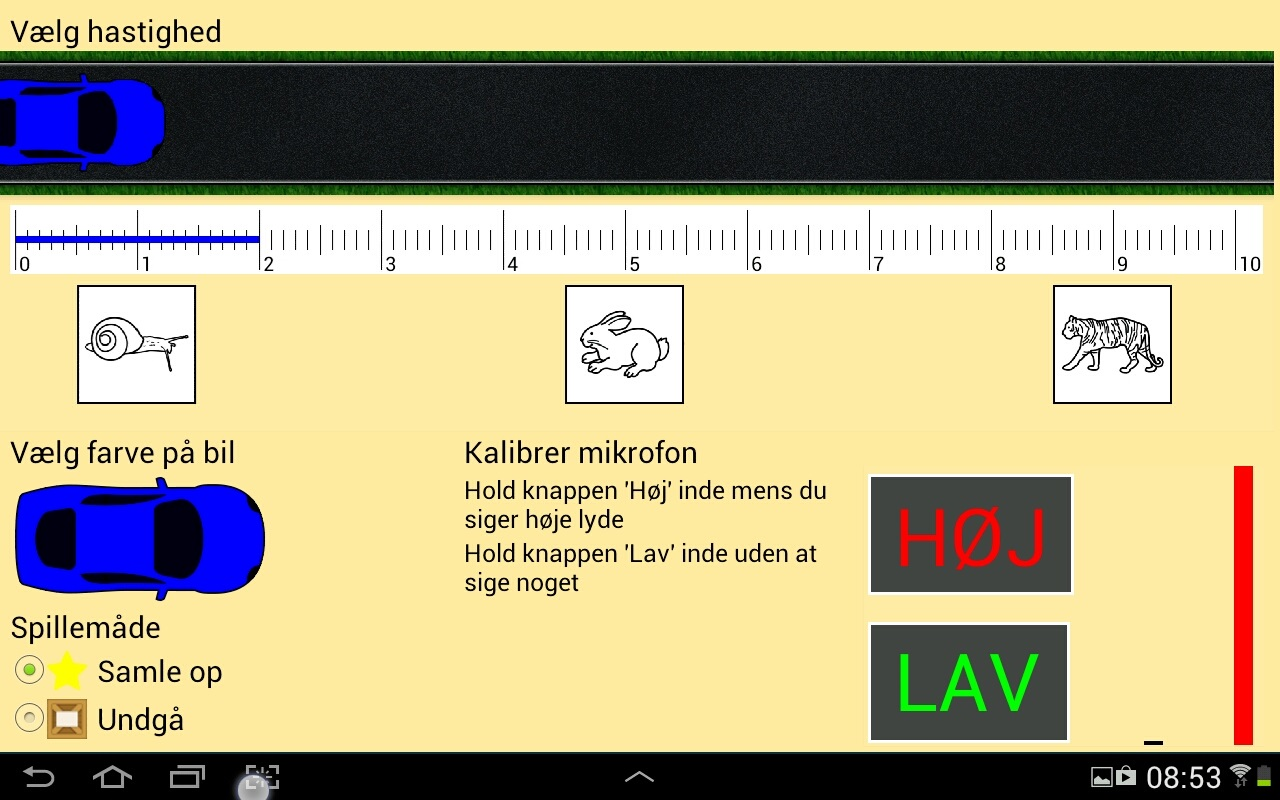
\includegraphics[width=\textwidth]{settings_s4}
\caption{The complete settings window}
\label{settings_s4}
\end{figure}

\subsection{Buttons and sounds}\label{s4_buttonsounds}
Another requirement that introduced changes to the application was \cref{sprint4_buttonspeak}.
All buttons now have to say their text when pressed and events need to have a sounds associated.

It was also a request to make the buttons look more like buttons visually.
The changes to the appearance can be seen on \cref{Buttons}, where \cref{old} shows the old appearance (where a button was only the text) and \cref{new} shows the new appearance (where a border and background color has been added), making the button resemble a traditional button more.

\subsection{ProfileSelector}
As of this sprint, \lstinline|giraf-component| library now provides a \lstinline|GButtonProfileSelect| class, to overcome a change in how profiles are switched.
Previously, a profile was selected in launcher, whenever an app is opened.
Now launcher has a currently active profile, which is the one provided when an app is opened.
Due to this, all apps must now provide an option of selecting another profile, using \lstinline|GButtonProfileSelect|.

\begin{figure}
\begin{subfigure}{0.5\textwidth}
\centering

\includegraphics[width=\textwidth]{oldButton}
\caption{The old appearance of the button}
\label{old}
\end{subfigure}
~
\begin{subfigure}{0.5\textwidth}
\centering

\includegraphics[width=\textwidth]{newButton}
\caption{The new appearance of the button}
\label{new}
\end{subfigure}
\caption{Changes in appearance of buttons}
\label{Buttons}
\end{figure}